\chapter{Modelling}
\section{Introduction}
Let's consider a cellular network consisting of the following modules:
\begin{itemize}
   \item \textbf{A Web Server}, which generates data in the form of packets, to be more precise, UserPackets, that is a defined type of packet which includes a \texttt{start\_time} field and its interface (named \texttt{UserPacket\_m}) includes a getter/setter method to update this field.
   
   The size of each packet is randomly generated in a uniform way, since the service demand has to be uniform.
   
   Each packet is scheduled according to an exponential RV, since the packet interarrival time has to be exponential.
   \item \textbf{An Antenna}, which includes a certain number of FIFO queues, one for each user. It stores the generated packets and send them in a unicast way according to the Round Robin policy (which is described in the next section). 
   \item \textbf{A Mobile Station}, which personifies a generic user connected to its own queue on the antenna. On each timeslot it sends a channel quality indicator (CQI), which is a number between 1 and 15 that determines the number of bytes that the antenna can pack into a Resource Block (RB).
   
   CQIs are integer RVs generated according the following scenarios:
   
   \begin{enumerate} 
    \item Uniform, the generated number is a uniform RV.
    \item Binomial, the generated number is a binomial RV
    \end{enumerate}
    
    Each Mobile Station computes some statistics: slotted throughput (related to each time slot) and response time of received packets.
\end{itemize}

\noindent The \texttt{CellularNetwork.ned} file shows how the previous modules are connected to obtain the network. 
Since frames are sent in a unicast way, there are multiple instances of the Web Server module, one for each Mobile Station, seeded in a different way.

\noindent The obtained network is the following: 
\begin{figure}[H]
  \centering
  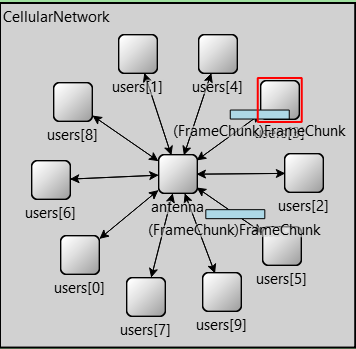
\includegraphics{images/network_simulations}
  \caption{Simulated Network (omnet++)}
  \label{fig:simulated_network}
\end{figure}



\section{Frame Chunks}

\section{Schedulers}
	\subsection{Round-Robin Frame Fill}
	\subsection{Best CQI based Frame Fill}